
\subsection*{\textbf{Question 1.d}}
\begin{quote}

\textbf{Problem}
\begin{quote}
Write a code that does the Kuiper’s test on your random numbers (see tutorial
8) and make the same plot as for the KS-test.
\end{quote}

\textbf{Solution} 
\begin{quote}
The implementation of the Kuiper test does simmilar to the KS-test require a numerical approximation of the CDF for the kuiper statistics. The CDF of the kuiper staistic is given by, 
\begin{equation}
P_{kuiper}( \lambda) =  1 - 2  \sum_{j=1}^{\infty} (4j^2 \lambda^2-1) e^{-2j^2 \lambda^2 }
\end{equation}

here the sum is negligible compared to the machine error if $\lambda < 0.4$. In this case the numerically approximation thus consist of simply returning 1.  If $\lambda > 0.4$ then the sum is approximated by calculating the first 100 terms of the sum, as this should be more than enough for the sum to converge. \footnote{In theory less terms should be more than enough. The evaluation of the sum could therefore stop early by checking for a required precision. This is however not implemented as summing 100 terms is cheap. } 

The kuiper test and the CDF are implemented in the shared module .\texttt{./Code/mathlib/statistics.py}, which is located on page ... .The code that creates the plots and the plots self can be found below.  This code does make use of \textbf{astropy} to compare self written implementation with the implementation of astropy. 
\end{quote}

\textbf{Code - Plots}

\begin{quote}
The code for generating the two plots in which the kuiper test is performed. The imports are not explicit shown but can be shown on page ..., where the code of the full assignment is displayed. The comments give an overview of the imports used. 
\lstinputlisting[firstline=167,lastline=197]{./Code/assigment_1.py}
\end{quote}

\textbf{Code - Output plot(s)}
\begin{quote}
\begin{figure}[!ht]
\centering
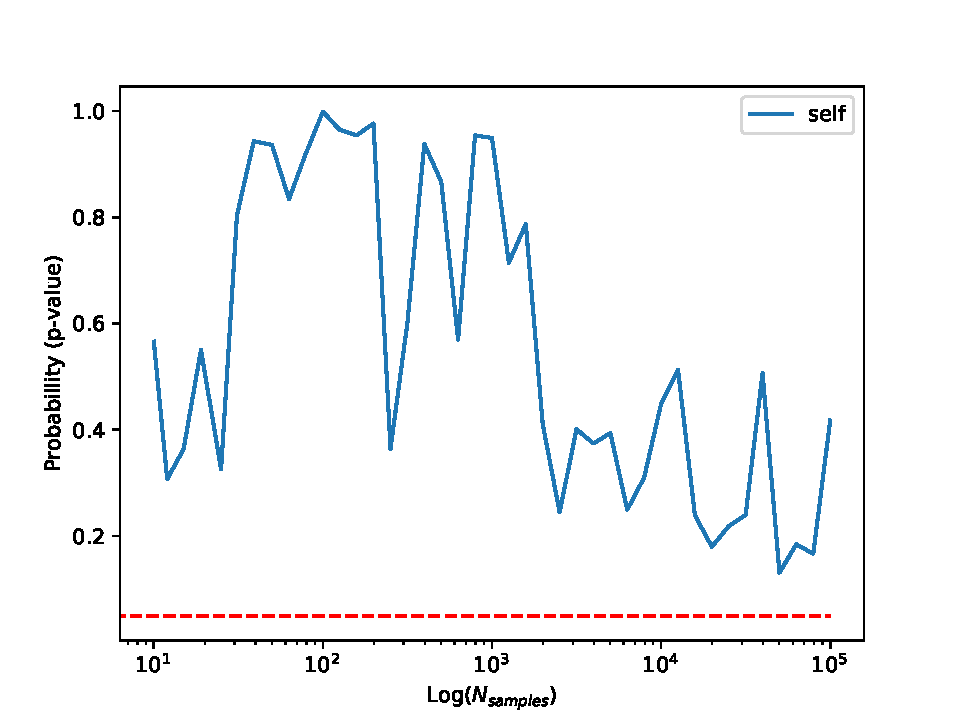
\includegraphics[width=12cm, height=7.5cm]{./Plots/1_plot_kuiper_test_self.pdf}
\caption{The P-value produced by the kuiper test against the number of samples on which the kuiper-test is performed for the self written RNG. The red line indicates the line of $ p = 0.05$. A point \textbf{below} there  line would suggests that there is enough statistical evidence to reject the (null) hypothesis that the data is normal distributed. The plot shows that the RNG always passes kuiper test. IT can however be seen that the value of the statistic stays lower for a significant amount of samples ($ N_{samples} > 10^4$). This might indicate that there is flaw in the random number generator.}
\end{figure}

\begin{figure}[!hb]
\centering
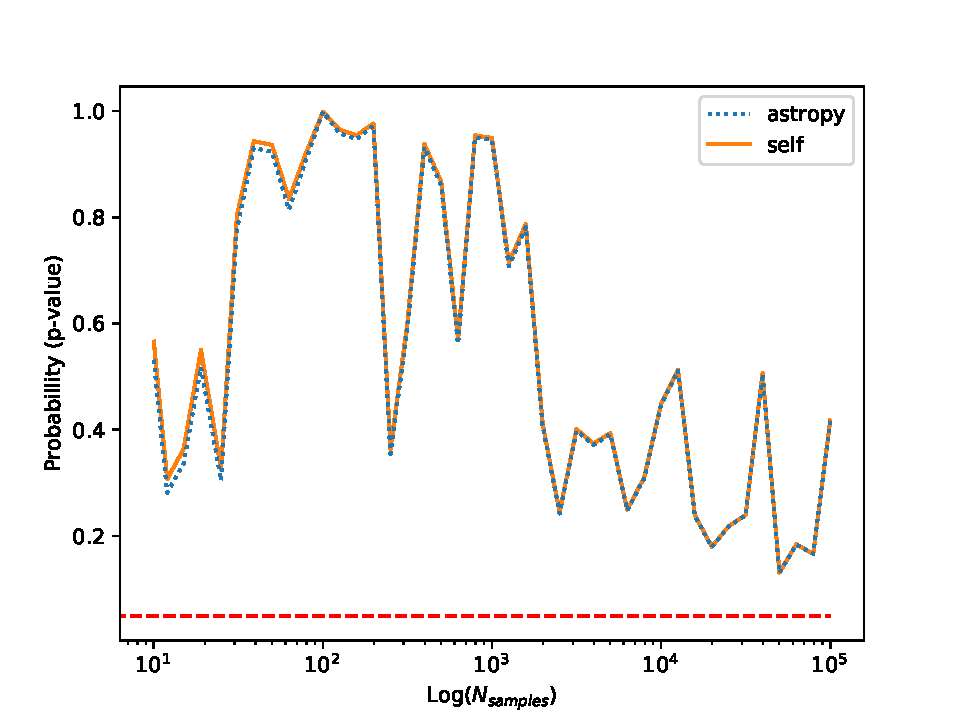
\includegraphics[width=12cm, height=7.5cm]{./Plots/1_plot_kuiper_test_self_astropy.pdf}
\caption{The P-value produced by the kuiper test against the number of samples on which the kuiper-test is performed for the self written RNG. The red line indicates the line of $ p = 0.05$. A point \textbf{below} there  line would suggests that there is enough statistical evidence to reject the (null) hypothesis that the data is normal distributed. The plot shows that the self written implementation deviates from the astropy implementation at the start, similar to what happend in the KS-test.   }
\end{figure}

\end{quote}



\end{quote}

\newpage

%\textbf{Code - output } 
%\begin{quote}
% The code that produces the output.
%\lstinputlisting{./code/assigment1_a.py}
%\end{quote}

%\textbf{Code - helper } 
%\begin{quote}
%The code for the Poisson distribution and the factorial function.  
%\lstinputlisting[firstline=2,lastline=46]{./code/mathlib/utils.py}
%\end{quote}


%\textbf{Output}
%\begin{quote}
%The output produced by \textsf{/code/assigment1\_ a.py} 
%\lstinputlisting{./output/assigment1_a_out.txt}
%\end{quote}
\newpage











